\documentclass{article}

\usepackage[spanish]{babel}
\usepackage[numbers,sort&compress]{natbib}
\usepackage[T1]{fontenc}
\usepackage[ansinew]{inputenc}
\usepackage{graphicx}
\usepackage{url}
\usepackage{caption}
\usepackage{subcaption}
\usepackage{float}

\title { M\'etodo Monte-carlo}
\author{Oscar Qui\~nonez}

\begin{document}

\maketitle
 
\section{Objetivo}\label{met}

Como parte del proyecto 5 se utiliza el m\'etodo Monte-carlo en el que se busca el tama\~no de la muestra que se requiere para conocer el lugar que ocupan hasta siete decimales generados por una integral que previamente fue ejecutada en el software Wolfram Alpha.

\section{Metodolog\'ia}\label{met}

Para esta simulaci\'on se requiri\'o el uso de R en su versi\'on 4.0.2, adem\'as del uso de un c\'odigo \cite{satuelisa} como base para generar distintas variaciones de este y obtener as\'i una rutina de 100 repeticiones para valores de 100, 1000, 10000, 100000 y 1000000 como tama\~no de muestra. Mediante el uso del m\'etodo Monte-carlo se calcul\'o la diferencia entre el valor real y el estimado para conocer as\'i el margen de error que existe entre ellos.

\section{Resultados y Discusi\'on}\label{res}

Al obtener los resultados de la rutina \cite{yo} se puede deducir que mientras mayor sea el valor en el tama\~no de la muestra mas nos acercamos al valor real de la integral que tomamos como referencia en Wolfram-Alpha, es decir la precisi\'on esta absolutamente relacionada con la cantidad de d\'igitos en la muestra pues se pueden obtener hasta 4 decimales para 1000000, lo que supone una mayor aproximaci\'on al valor real.
En la figura 1 que se muestra a continuaci\'on, se presenta un diagrama de caja-bigote en la que la precisi\'on se ve representada como el \'area que se encuentra por debajo de cada una de las l\'ineas de colores, como indica la leyenda ubicada en el extremo superior derecho. Esta nos indica que efectivamente mientras mayor sea el valor de la muestra, el margen de error se ver\'a reducido y por eso las l\'ineas roja y verde est\'an muy cercanas entre ellas.

\begin{figure}
  \centering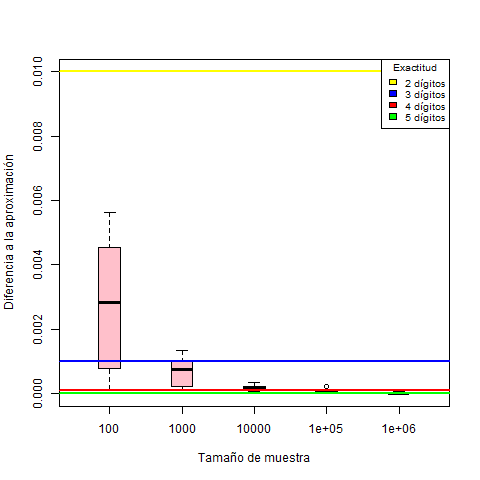
\includegraphics[scale=0.7]{Grafica1.png}
  \caption{Diagrama de caja-bigote en la que se observan las aproximaciones al valor real.}
  \label{fig}
\end{figure}

\newpage

\section{Conclusi\'on}

Existe una relaci\'on directa entre la aproximaci\'on al valor real de la integral y el valor de la muestra con la que se calcul\'o, pues mientras mayor sea este \'ultimo, m\'as decimales nos generar\'a y mayor ser\'a la cercan\'ia de los valores, como se vio representada en las l\'ineas de la figura1.  El m\'etodo Monte-carlo es muy \'util en este tipo de experimentos pues nos permite usar expresiones matem\'aticas complejas (en este caso una integral) para aproximarnos a valores exactos que de otra manera ser\'ian demasiado tardados para valores muy grandes sin el uso de una computadora.

\section{Reto1}

El reto consiste en usar la t\'ecnica de Kurt \cite{kurt} para estimar el valor de $\pi$ mas exacto posible, sabiendo que la precisi\'on en los decimales est\'a relacionada al tama\~no de la muestra, como fue demostrado en la tarea base. Este m\'etodo se basa en la determinaci\'on del valor de $\pi$ a trav\'es del \'area de un c\'irculo y un cuadrado en la que la relaci\'on puede expresarse como $\pi$/4. En la figura 2 se muestran dos diagramas para el representar el valor exacto de $\pi$, donde se indican los valores generados y comparados con los esperados (los que caen en la banda de color azul), as\'i como los valores generados en comparaci\'on con los decimales utilizados, pues como ya se mencion\'o anteriormente mientras mas valores existan mas se aproxima al valor exacto. 

\begin{figure}
  \centering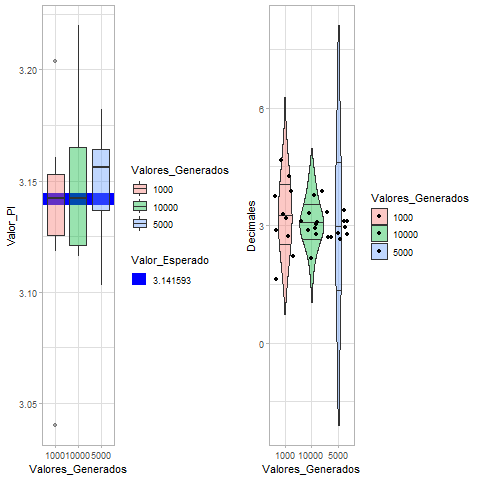
\includegraphics[scale=0.6]{Grafica2.png}
  \caption{Representacion entre los valores generados contra el valor esperado.}
  \label{fig}
\end{figure}

\newpage
\bibliography{tareacinco}
\bibliographystyle{unsrtnat}

\end{document}
